%! Author = Saeid Yazdani
%! Date = 4/25/2024


\section{\acs{VDUT} Prototype}
\label{sec:vdut-prototype}

The \ac{DUT} under investigation requires six voltage rails
for its core and various peripherals.
In an ideal scenario, a \ac{VDUT} should also have load and measurement circuits
for each voltage rail according to the concept proposed in
\autoref{sec:vdut-concept}.

Furthermore, as stated in \autoref{subsec:dut_description}, the \ac{DUT} is
built on a small \ac{LFBGA} package with a total area of
\SI{289}{\milli\meter\squared}.
This is indeed a relatively small area to realize all \ac{VDUT} requirements,
given that each voltage rail will require load switching, voltage and
current monitoring where each of these sub-circuits will require a few
passive components to be configured and operated as intended.

\subsection{Choice of Components}
\label{subsec:vdut-choice-of-components}

Fortunately, modern components with very small footprints allow
complex circuits within a limited area, making the realization of
\ac{VDUT} concept not out of reach.

The key components of the \ac{VDUT} are the amplifiers, load switches
and coaxial connectors for signal transmission.
The following components were selected to be used in
prototyping a \ac{VDUT} according to the concept requirements:

\begin{itemize}[topsep=8pt,itemsep=4pt,partopsep=4pt, parsep=4pt]

    \item \textbf{Amplifier:} ADA4817-1, a
    unity-gain stable, high-speed, low-noise, voltage feedback
    amplifier with \ac{FET} inputs \autocite{analogdevices:ADA4817}.

    \begin{itemize}[topsep=8pt,itemsep=4pt,partopsep=4pt, parsep=4pt]
        \item Dimensions: \SI{3}{\milli\meter} (L) x \SI{3}{\milli\meter} (W)
        x \SI{0.75}{\milli\meter} (H)
        \item Slew rate: \SI{870}{\volt\per\micro\second}
        \item Input bias current: \SI{2}{\pico\ampere}
        \item Operating temperature range:
        \SI{-40}{\degreeCelsius} to \SI{105}{\degreeCelsius}
    \end{itemize}


    \item \textbf{Load Switch:} CSD13380F3, N-Channel
    \acs{MOSFET} with ultra-small footprint and low on-resistance
    ~\autocite{ti:CSD13380F3-datasheet}.

    \begin{itemize}[topsep=8pt,itemsep=4pt,partopsep=4pt, parsep=4pt]
        \item Dimensions: \SI{0.73}{\milli\meter} (L) x \SI{0.64}{\milli\meter} (W)
        x \SI{0.36}{\milli\meter} (H)
        \item ON-Resistance: \SI{63}{\milli\ohm}
        \item Drain-Source Voltage: \SI{12}{\volt}
        \item Drain-Source Current: \SI{3.6}{\ampere}
        \item Operating temperature range:
        \SI{-55}{\degreeCelsius} to \SI{150}{\degreeCelsius}
    \end{itemize}

    \item \textbf{Coaxial Connector:} W.FLCL331, miniature surface mount
    coaxial connector \autocite{hirose:wflcl331-datasheet}.

    \begin{itemize}[topsep=8pt,itemsep=4pt,partopsep=4pt, parsep=4pt]
        \item Dimensions: \SI{2.0}{\milli\meter} (L) x \SI{2.0}{\milli\meter} (W)
        x \SI{0.85}{\milli\meter} (H)
        \item Frequency range: Up to \SI{6}{\giga\hertz}
        \item Breakdown voltage: \SI{200}{\volt} \acs{DC}
        \item Operating temperature range:
        \SI{-40}{\degreeCelsius} to \SI{90}{\degreeCelsius}
    \end{itemize}

\end{itemize}

The rest of the components will be passive resistors, capacitors and inductors
in \emph{0603} (\SI{1.6}{\milli\meter} x \SI{0.8}{\milli\meter})
package.
The load components will be in \emph{0805} (\SI{2.0}{\milli\meter} x
\SI{1.25}{\milli\meter})
package since they provide
a better power dissipation than smaller packages and more manageable during
field rework.

\subsection{Production of \acs{VDUT} Prototype}
\label{sec:vdut-first-variant-prototype}

To demonstrate the viability of the \ac{VDUT} concept, a prototype
was designed, produced and tested.
It contains all six \ac{DUT} core and peripheral supply rails
controlled by CSD13380F3 \ac{FET}, connected to a single amplifier.
This variant focuses solely on voltage sensing of supply rails switched
by the \acp{FET}.

This \ac{VDUT} is a four-layer design and
\autoref{fig:vdut-cad-drawing-top-bot} shows the top layer where components are
located and the bottom layer where the solder pads for \ac{BGA} balls are
located.

The produced prototype of a \ac{VDUT} is presented
in \autoref{fig:vdut-first-prototype-production} where the components,
control and supply wires and solder balls to the bottom side are
visible.

\begin{figure}[htbp]
    \centering
    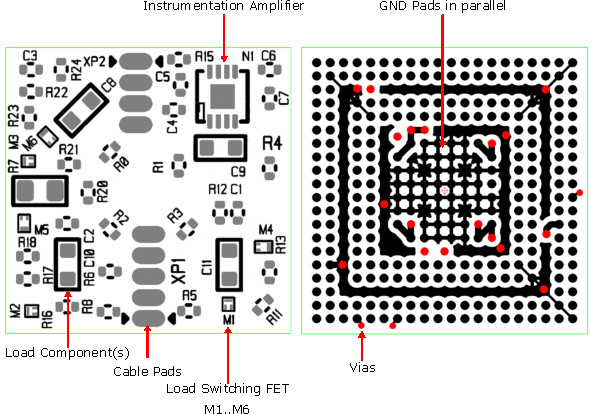
\includegraphics[width=\linewidth,height=0.62\textheight,keepaspectratio]
    {figures/vdut/vdut-cad-top-bot}
    \caption[\acs{CAD} Drawing of \acs{VDUT} Concept]{
        \ac{CAD} Drawing of \ac{VDUT} concept. \textbf{Left:}
        small instrumentation amplifier, FemtoFET\texttrademark{} switches,
        test loads and connecting pads for control and measurement cables are
        visible on the top layer.
        \textbf{Right:} BGA pads and vias on the bottom layer.
        Ground and supply pins are in parallel with the same number of pins
        as in the real \ac{DUT}.}
    \label{fig:vdut-cad-drawing-top-bot}
\end{figure}

\begin{figure}[htbp]
    \centering
    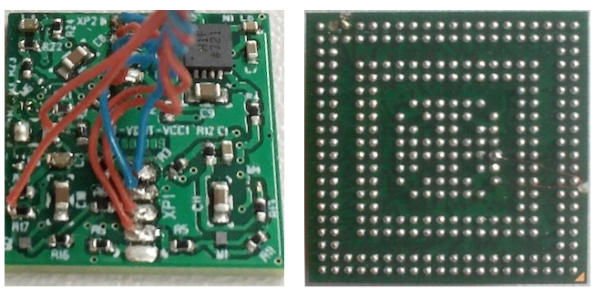
\includegraphics[width=\linewidth,height=0.62\textheight,keepaspectratio]
    {figures/vdut/vdut-real-top-bot}
    \caption[Prototype of \acs{VDUT} Concept]{
        Produced prototype of the \ac{VDUT} concept as presented in
        \autoref{fig:vdut-cad-drawing-top-bot}.
        Key components such as instrumentation amplifier, FemtoFET\textcopyright{}
        on the top side (left) and solder balls on the bottom side (right)
        are visible. For the first prototype a simple solder pad is used instead of coaxial cables.}
    \label{fig:vdut-first-prototype-production}
\end{figure}

\subsection{\acs{VDUT} Initial Test Setup}
\label{sec:vdut-first-variant-initial-test-setup}

\autoref{fig:vdut-in-loadboard-socket} shows the \ac{VDUT} sitting inside the
test socket in the \ac{ATE} environment.
The accompanying control box for \ac{VDUT} that provides both positive and
negative supply rails for the onboard amplifier as well as a microcontroller
to trigger load switches is shown in \autoref{fig:vdut-control-box}.
The dual supply design for the voltage sense amplifier allows the output to
swing both above and below ground, enabling the ability to capture overshoot
and undershoots even under reference potential.

\begin{figure}[htbp]
    \centering
    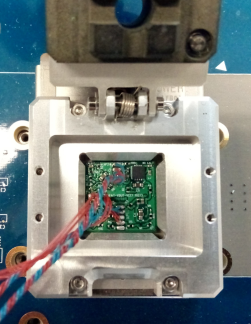
\includegraphics[scale=1]
    {figures/vdut/vdut-protoype-in-socket-resized}
    \caption[\acs{VDUT} Prototype in Socket]{
        \ac{VDUT} Prototype inserted into the socket on the load board.}
    \label{fig:vdut-in-loadboard-socket}
\end{figure}

\begin{figure}
    \centering
    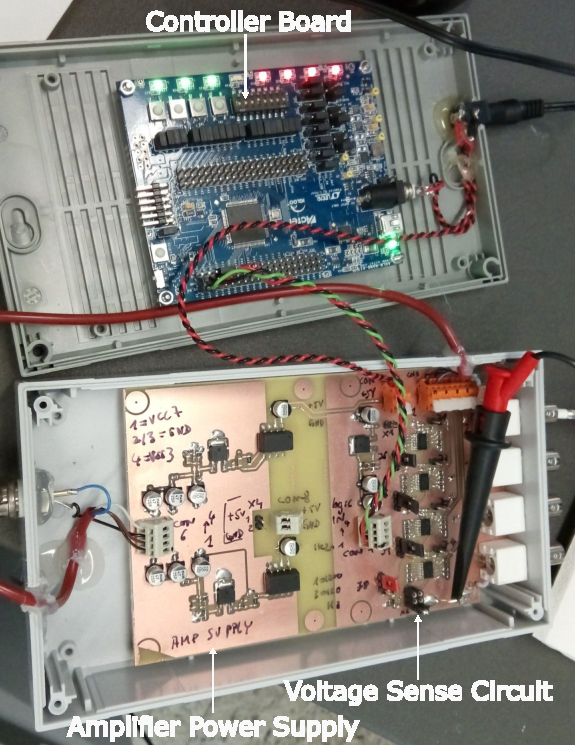
\includegraphics[scale=1]
    {figures/vdut/vdut-control-box}
    \caption[\acs{VDUT} Control Box]{
        The control box of \ac{VDUT} where positive and negative supply rails
        for amplifier and \acs{FET} switch control lines are located.
    }
    \label{fig:vdut-control-box}
\end{figure}

\subsection{Measurement Results Using Prototype \ac{VDUT} }
\label{sec:vdut-measurements-using-prototype}

First measurement with the \ac{VDUT} used a capacitive load of
\SI{10}{\micro\farad} to stimulate the \SI{1.3}{\volt} supply rail.
For these measurements, no support capacitance was on the load board.

\autoref{fig:vdut-result-1v3-10uF} shows the measurement result captured
by an oscilloscope.
The blue trace at the top represents the gate signal of the load \acs{FET}
where a high signal indicates current flow through the socket.
The red trace illustrates the rail waveform as monitored by the \ac{VDUT}.
The overall measurement demonstrates that activating a capacitive load
(similar to that with a switching DUT) results in a voltage drop below
\SI{1}{\volt} of approximately \SI{500}{\milli\volt}.
This drop could potentially cause disruptions to the DUT during testing.
The voltage recovers within \SI{100}{\micro\second}, but during testing, this
includes a significant portion of a test program sequence.

\begin{figure}
    \centering
    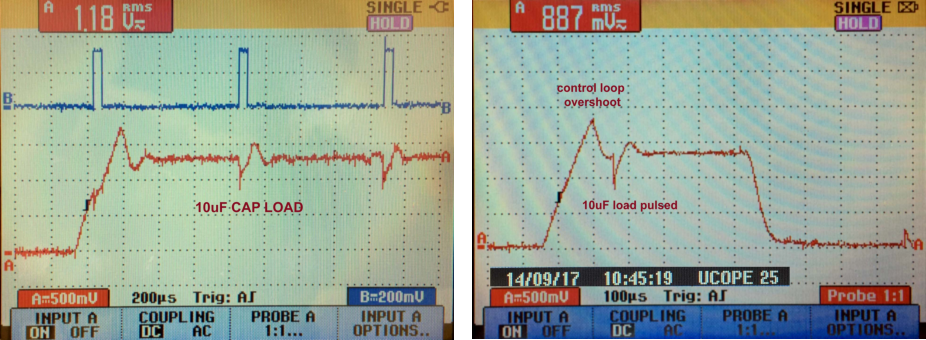
\includegraphics[width=\linewidth,height=0.62\textheight,keepaspectratio]
    {figures/vdut/vdut-result-1v3-10uF}
    \caption[\acs{VDUT} Stimulating \acs{DPS} with Capacitive Load]{
        \textbf{Left:} \ac{VDUT} Stimulating the \SI{1.3}{\volt} rail of the \ac{ATE}'s
        \ac{DPS} unit with a \SI{10}{\micro\farad} capacitive load
        as seen from the onboard voltage sense amplifier.
        \textbf{Right:} Increased time base for more pulse resolution.
    }
    \label{fig:vdut-result-1v3-10uF}
\end{figure}

The same supply rail was tested again with a resistive load of \SI{4.7}{\ohm}
and the resulting waveforms are presented in \autoref{fig:vdut-result-1v3-4R7}.
This measurement reveals that releasing the load leads to an immediate increase
in the voltage rail.
This shows that the \ac{DPS} control loop is too slow to immediately recognize
the new situation in the load change.
As soon as the load is activated again, we observe another voltage undershoot.

\begin{figure}[htbp]
    \centering
    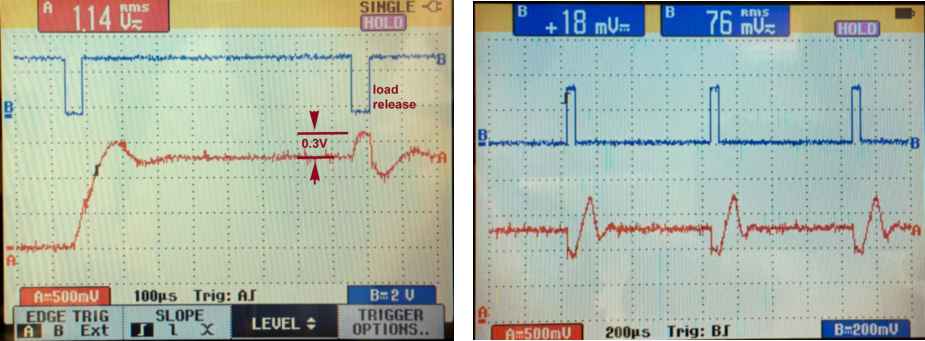
\includegraphics[width=\linewidth,height=0.62\textheight,keepaspectratio]
    {figures/vdut/vdut-result-1v3-4R7}
    \caption[\acs{VDUT} Stimulating \acs{DPS} with Resistive Load]{
        \textbf{Left:} \ac{VDUT} Stimulating the \SI{1.3}{\volt} rail of the \ac{ATE}'s
        \ac{DPS} unit with a \SI{4.7}{\ohm} resistive load
        as seen from the onboard voltage sense amplifier.
        \textbf{Right:} Same resistive test with shorter current pulses.
    }
    \label{fig:vdut-result-1v3-4R7}
\end{figure}

By adding a \SI{50}{\micro\farad} support capacitance on the load board at
designated places near the socket and repeating the resistive load test, a
large voltage overshoot is observed during the programmed supply rail ramp-up
phase, as shown in \autoref{fig:vdut-result-1v3-4R7-added-50uF-bypass}.

\begin{figure}[htbp]
    \centering
    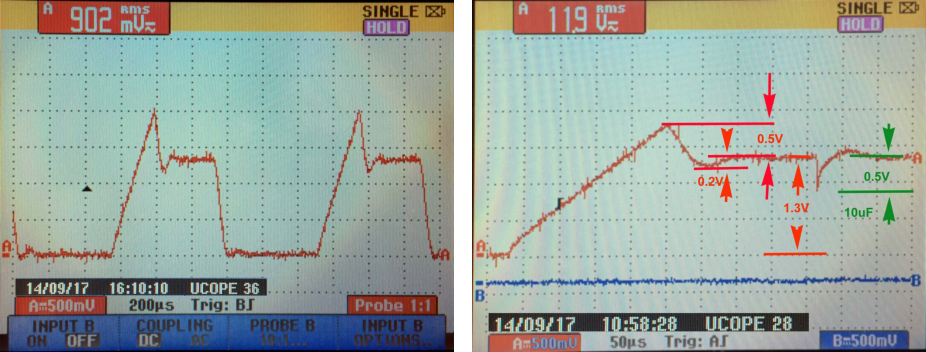
\includegraphics[width=\linewidth,height=0.62\textheight,keepaspectratio]
    {figures/vdut/vdut-result-1v3-4R7-added-50uF-bypass}
    \caption[\acs{VDUT} Stimulating with Resistive Load and Bypass Capacitor]{
        \textbf{Left:} \SI{1.3}{\volt} rail overshoot
        with a \SI{4.7}{\ohm} load and added \SI{50}{\micro\farad}
        bypass capacitor on the load board near the socket,
        as seen from the onboard voltage sense amplifier.
        \textbf{Right:} Lower time base of the same signal for studying the
        waveform.
    }
    \label{fig:vdut-result-1v3-4R7-added-50uF-bypass}
\end{figure}

\subsection{Lessons Learned from \ac{VDUT}}
\label{sec:vdut-lessons-learned-first-prototype}

Although the \ac{VDUT} stimulating and
capturing responses of \ac{ATE}'s \ac{DPS} module performed very well,
there were major points that can be improved:

\begin{itemize}[topsep=8pt,itemsep=4pt,partopsep=4pt, parsep=4pt]
    \item \textbf{Insertion mechanism: }
    The insertion of the actual \ac{DUT}
    into the test socket involves pushing the chip into the socket and closing
    the socket lid to generate an even amount
    of force to make sure the contact between socket pogo pins and \ac{BGA}
    pads are reliable.
    This of course works very well with the flat and hard surface of a packaged
    \ac{IC}.

    \item \textbf{Choice of components: }
    The CSD13380F3 switching \ac{FET} was selected due to its very small
    \ac{LGA} footprint (\autoref{fig:csd13380-mechanical-dimensions}), allowing
    the inclusion of more than one supply rail per \ac{VDUT}.
    In case of manual assembly, soldering this component is quite challenging.

    \item \textbf{Use of coaxial cables: }
    Using miniature coaxial connectors can improve noise rejection and having
    mating receptacles on the \ac{PCB} will increase connection reliability.

\end{itemize}

\begin{figure}[h!]
    \centering
    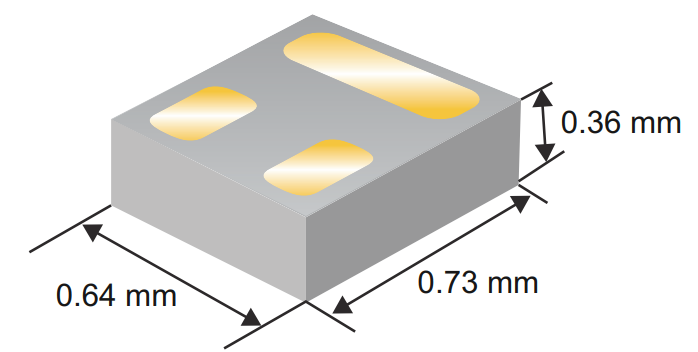
\includegraphics[width=0.5\textwidth]
    {figures/vdut/csd13380f3_dimensions}
    \caption[Dimensions of CSD13380f3 \acs{FET} Switch]{
        Mechanical dimensions of the CSD13380f3
        \autocite{ti:CSD13380F3-datasheet}.
    }
    \label{fig:csd13380-mechanical-dimensions}
\end{figure}

\subsection{Improved \ac{VDUT}}
\label{sec:vdut-improved-prototype}

Based on the first measurement experience with \ac{VDUT} and previously
discussed points for improvement, a new set of \ac{VDUT} was developed.

By dedicating each \ac{VDUT} for a specific supply rail, a more relaxed
selection of components and the ability to add extra circuitry could be
achieved.
This frees space to use larger switches instead of the CSD13380F3 and use of
miniature-sized coaxial connectors~\autocite{hrs:wfl2} as shown
in \autoref{fig:vdut2-components}.

\begin{figure}[htbp]
    \centering
    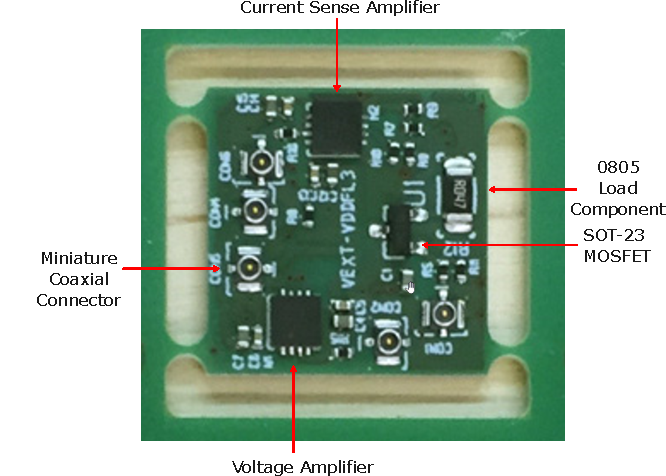
\includegraphics[width=\textwidth]
    {figures/vdut/vdut2-components}
    \caption[Components of the Improved \acs{VDUT}]{
        Components of the improved \ac{VDUT}.
    }
    \label{fig:vdut2-components}
\end{figure}

Moving to automated assembly enables the cost-effective production of multiple
\ac{VDUT} variants (per supply rail) on a single panel as depicted in
\autoref{fig:vdut2-variants}.

\begin{figure}[htbp]
    \centering
    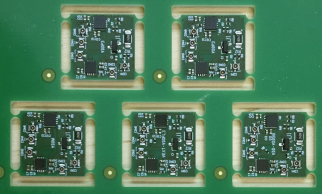
\includegraphics[width=\linewidth,height=0.62\textheight,keepaspectratio]
    {figures/vdut/vdut2-variants}
    \caption[Variants of improved \acs{VDUT}]{
        All variants of the improved \acs{VDUT} produced on a single \ac{PCB}
        panel.
    }
    \label{fig:vdut2-variants}
\end{figure}

\begin{figure}[h]
    \centering
    \printfitgraphics[0.62\textheight]{figures/vdut/vdut2-in-socket_closeup}
    \caption[Improved \acs{VDUT} in Socket]{
        Improved \acs{VDUT} with connected \acs{SMT} small coaxial cables next to the socket.
    }
    \label{fig:vdut2-in-socket}
\end{figure}

